\documentclass[]{article}
\usepackage[T1]{fontenc}
\usepackage{subfigure}
\usepackage{lmodern}
\usepackage{amssymb,amsmath}
\usepackage{ifxetex,ifluatex}
\usepackage{fixltx2e} % provides \textsubscript
% use microtype if available
\IfFileExists{microtype.sty}{\usepackage{microtype}}{}
\ifnum 0\ifxetex 1\fi\ifluatex 1\fi=0 % if pdftex
  \usepackage[utf8]{inputenc}
\else % if luatex or xelatex
  \usepackage{fontspec}
  \ifxetex
    \usepackage{xltxtra,xunicode}
  \fi
  \defaultfontfeatures{Mapping=tex-text,Scale=MatchLowercase}
  \newcommand{\euro}{€}
\fi
% Redefine labelwidth for lists; otherwise, the enumerate package will cause
% markers to extend beyond the left margin.
\makeatletter\AtBeginDocument{%
  \renewcommand{\@listi}
    {\setlength{\labelwidth}{4em}}
}\makeatother
\usepackage{enumerate}
\usepackage{graphicx}
% We will generate all images so they have a width \maxwidth. This means
% that they will get their normal width if they fit onto the page, but
% are scaled down if they would overflow the margins.
\makeatletter
\def\maxwidth{\ifdim\Gin@nat@width>\linewidth\linewidth
\else\Gin@nat@width\fi}
\makeatother
\let\Oldincludegraphics\includegraphics
\renewcommand{\includegraphics}[1]{\Oldincludegraphics[width=\maxwidth]{#1}}
\ifxetex
  \usepackage[setpagesize=false, % page size defined by xetex
              unicode=false, % unicode breaks when used with xetex
              xetex]{hyperref}
\else
  \usepackage[unicode=true]{hyperref}
\fi
\hypersetup{breaklinks=true,
            bookmarks=true,
            pdfauthor={Authors: Matthew Russell, Hashem Nasarat, and Juan Carlos Montemayor Elosua},
            pdftitle={Patching in Parallel: A Simplified Approach to Version Control},
            colorlinks=true,
            urlcolor=blue,
            linkcolor=magenta,
            pdfborder={0 0 0}}
\setlength{\parindent}{0pt}
\setlength{\parskip}{6pt plus 2pt minus 1pt}
\setlength{\emergencystretch}{3em}  % prevent overfull lines
\setcounter{secnumdepth}{0}

\title{Patching in Parallel: A Simplified Approach to Version Control}
\author{Authors: Matthew Russell, Hashem Nasarat, and Juan Carlos Montemayor
                Elosua}
\date{Date: Dec 11, 2012}

\begin{document}
\maketitle

\section{Abstract}

A version control system (VCS) tracks the history of a filesystem and
allows users to create snapshots at different points in time and move
between them at will. They are typically utilized in software projects
to manage parallel lines of development and to combine different
versions of a file in a way that is predictable and present conflicting
changes to user.

We present our model of a simplistic VCS and show how the chosen
representation of patches enables a simple method for conflict detection
and resolution when combining lines of development. Previous work on
version control systems either neglects to provide an algorithm for
conflict detection or offers an alternative representation and
consequently, a more complex solution to the conflict detection problem.
Utilizing our detection algorithm, we can easily define the rebase
operation for replaying changes onto another line of development in a
concise and clear manner.

\section{Intro}

Version control systems are vital tools utilized by Computer Scientists
and Software Engineers. Surprisingly, there is little academic
literature on this subject and the few papers that are found typically
leave readers without a full understanding of the problems and solutions
necessary to create a working VCS. Because many VCSs lack a complete or
convoluted specification, users experience strange behavior such as
incorrect auto-merging and problems in conflict detection. By describing
the representation of changes to files in a complete manner and the
strategies used to merge parallel lines of development, users can rest
assured that the tools they use will behave predictably in any
situation.

In examining the academic literature for previous work, we draw a
distinction between two differing notions of version control.
State-based systems such as git rely on storing the contents of file
system or pointers to the contents at each snapshot in time. Previous
work on state based systems includes a detailed understanding of the
representation of these snapshots and how to efficiently manage large
numbers of files. However, there are relatively few descriptions of how
more complicated operations such as merge, rebase, and conflict
detection are implemented in practice.

Change-based systems only store the changes to the files that led from
the previous snapshot to the current one. There has been substantial
previous work on the subject of change-based VCSs, specifically
regarding how to changes in a filesystem can be represented and combined
(Roundy 2009). Darcs and Camp are built upon this patch theory. Patch
theory becomes increasingly complicated when reasoning about resolving
conflicts between patches because a patch can be a composition of
several previous patches and must be decomposed before conflict
detection can proceed (such complexities are admitted in Roundy 2009).

We have taken a different strategy by designing and implementing a
version control system that combines the repository representation of a
state-based approach with the representation of patches from a
change-based approach. At its core, we represent points in time as a
snapshot of the file system, but when determining the differences
between two snapshots, we expand on a subset of the Patch Theory
described by David Roundy. By viewing changes between states in this
way, we are able create a simplified version control system that is
functional, easy to reason about, and allows for exploration of the
challenging problems of conflict detection, rebase, and merge.
Implementing this model in Haskell allows us to verify our algebraic
laws using QuickCheck and leverage the Type Class feature to simplify
our algorithms for conflict detection.

This paper seeks to address a fundamental gap in academic literature on
version control systems by making the following contributions: * We
define a representation of changes between states in a filesystem as a
set of parallel patches which all reference a common initial state; * We
present a simple and easy to understand conflict detection algorithm to
merge two sets of parallel patches; * We provide a general algorithm for
rebasing two lines of parallel development which is simple to understand
and reason about; * We illuminate certain difficulties when considering
how to rebase when commits have multiple parents; * We provide a
reference implementation of our small but complete version control
system model, which is easy to reason about, and can be used as a
platform for future experimentation.

\section{Version Control Terminology}

In this section we will detail the common fundamental aspects of version
control.

\subsubsection{Diffs and Patches}

A \emph{diff}, as the unix \texttt{diff} command's man page states,
``compares files line by line.'' For example, if \texttt{a} and
\texttt{b} are files, \texttt{\$ diff a b} indicates the differences
between two files by showing:

\begin{itemize}
\item
  which lines are shared between \texttt{a} and \texttt{b} (no change),
\item
  which lines from \texttt{a} have been removed in \texttt{b}
  (deletions), and
\item
  which lines in \texttt{b} were not present in \texttt{a} (additions).
\end{itemize}

The output of \texttt{diff} is called a \emph{patch}, and it indicates
the changes made which changed \texttt{a} into \texttt{b}. A patch is
subdivided into multiple discrete groups of changes called \emph{hunks}
or \emph{change hunks} in the terminology of \texttt{diff}. Hunks
contain the offset in the file \texttt{a} in which a change occurred,
the lines that were removed, and the lines that were added (at this
offset).

Version control systems often use some notion of a patch to represent
changes in files at various points in time.

\subsubsection{Conflicts}

Patches can be applied to a file to repeat the changes described in the
patch to that file. However, when applying multiple patches to a file,
for example, patches P\_a and P\_b, P\_a may contain change hunks which
indicate changes that contradict with some change hunks in P\_b. These
contradicting change hunks are called \emph{conflicts}. Most version
control systems present the user with the conflicting change hunks for
resolution by hand.

A conflict occurs when two patches modify the same line in a file, and
the patches are not identical.

\subsubsection{Commits}

A \emph{commit} marks a state of the filesystem at a given time, and
represents a specific point in time of the filesystem. Users of a VCS
can move between states in time in the filesystem by moving between
commits. Commits have some sense of dependency on previous commits to
present a loose ordering on states of the filesystem.

\subsubsection{Branches}

A \emph{branch} is a one of multiple divergent lines of commits, rooted
at a least common ancestor commit (LCA). Often branches are used for
working on different features, or when multiple users are adding commits
to the same repository, as it keeps related changes together.

\subsubsection{Repository}

At the most basic level, a \emph{repository} is simply a collection of
commits. At a higher level, many VCSs also present a set of named
branches and other conveniences. In total, the repository represents the
entire history of the filesystem.

\subsubsection{Combining Changes}

Although branches are a convenient feature for separating groups of
commits, at some point it is necessary to combine the disparate changes
contained in various branches and combine two branches into one. Two
methods of combining changes are \emph{merge} and \emph{rebase}.

\begin{itemize}
\item
  Rebase: One branch, \emph{b1}, is replayed commit by commit on top of
  the end of another branch, \emph{b2}. Essentially this moves the point
  at which \emph{b1} diverged to the end of \emph{b2}, removes the
  divergence, and turns the two branches into one. The commit at the end
  of this new branch contains all the changes made in \emph{b1} and
  \emph{b2}.
\end{itemize}

\begin{quote}
Given two lines of development:
\end{quote}

\begin{quote}
\begin{figure}[Figure 1]
\centering
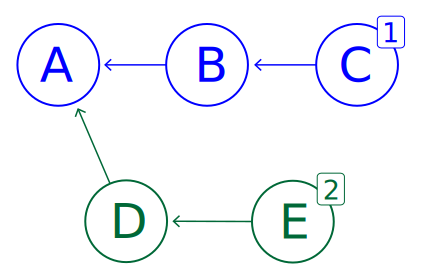
\includegraphics{img/hashem1.png}
\caption{}
\end{figure}
\end{quote}

\begin{quote}
A rebase of line ADE onto line ABC results in a repository
\end{quote}

\begin{quote}
\begin{figure}[Figure 2]
\centering
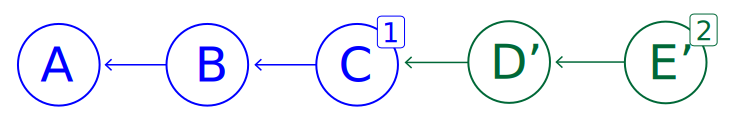
\includegraphics{img/hashem2.png}
\caption{}
\end{figure}
\end{quote}

\begin{itemize}
\item
  With merge, a new commit is created with two parents (the two commits
  from the separate lines of development). The total changes needed to
  go from the LCA to the two parents are combined and applied together,
  creating a commit with the combined changes. Since the new commit has
  two parents, two branches were combined into one.
\end{itemize}

\begin{quote}
\begin{figure}[Figure 3]
\centering
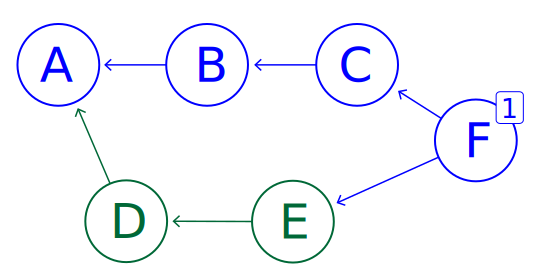
\includegraphics{img/mrg.png}
\caption{}
\end{figure}
\end{quote}

\section{Changes \& Conflict Detection}

This section defines a representation changes between two states as
patches in parallel and examines how conflict detection is simplified
under this model.

\subsection{The Patch}

We construct the precise notion of a patch, a difference between two
states of a file, in parts:

\subsubsection{Edit}

We represent a diff between two files as a list of \texttt{Edit}s where
an \texttt{Edit} has the following type:

\begin{verbatim}
data Edit t = C -- Copy current input line to output 
            | I t -- Insert argument line into output
            | D t -- Delete current input line which must match
                deriving (Show, Eq)
\end{verbatim}

The problem with representing changes as a list of \texttt{Edit}s is
that they can be quite large since: * the number of Cs + Ds = length
(original file) * the number of Cs + Is = length (new file)

\subsubsection{ChangeHunk}

We needed a way to represent changes to a file in a compact and discrete
manner, and the patch model from diff, worked nicely:

\begin{verbatim}
data ChangeHunk = ChangeHunk { offset :: Int
                    , old :: [String] -- Old lines
                    , new :: [String] -- New lines
                    }
\end{verbatim}

We convert changes expressed in list of Edits to lists of ChangeHunks
with the following:

\begin{verbatim}
editsToChangeHunks :: [Edit String] -> [ChangeHunk]
\end{verbatim}

Each \texttt{ChangeHunk} in output of \texttt{editsToChangeHunk}
references the line number in the original file. When group of
\texttt{ChangeHunk}s all reference the original file (in offset and old
lines), we consider these \texttt{ChangeHunk}s to be in parallel.
Alternatively, when each \texttt{ChangeHunk} in a sequence references
the state of the file after all preceding \texttt{ChangeHunk}s have been
applied, we consider these \texttt{ChangeHunk}s to be in sequence. We
use terminology from Roundy 2009, developed to build darcs.
Distinguishing between parallel and sequential \texttt{ChangeHunk}s (and
thus the following datatypes) will prove important later in this paper.

\subsubsection{PatchAction}

Again, we borrow the \texttt{PatchAction} datatype from Darcs, which
enables descriptions of more types of file modifications. Readers who
are familiar with Darcs might notice that this \texttt{PatchAction}
datatype enables removing and creating non-empty files. This change was
needed to overcome a conceptual impasse in which a
\texttt{CreateEmptyFile} and a \texttt{ChangeHunk} could not be in
parallel since the former necessarily must be applied first (this is the
case when a new file is created with contents).

\begin{verbatim}
data PatchAction = RemoveFile [String] -- File contents to delete
                 | CreateFile [String] -- File contents to add
                 | Change ChangeHunk
\end{verbatim}

Finally, we complete our notion of a \texttt{Patch} by associating a
\texttt{PatchAction} with a particular path:

\begin{verbatim}
data AtPath t = AP Path t

type Patch = AtPath PatchAction
\end{verbatim}

A set of parallel patches cannot all be directly applied to a single
point in time (list of files) because the act of applying one patch from
the set creates a new state which the remaining parallel patches may no
longer correctly reference. For instance, if \texttt{ChangeHunk} A adds
``functional'' at line 0 and \texttt{ChangeHunk} B adds the line
``programming'' at line 1 and we apply A before B, then B no longer
correctly references the original position in the file.

Instead of potentially adjusting offsets after every application, we can
put the parallel patches in sequence before application to the file
system. A trivial transformation of parallel patches to sequential
patches involves grouping the patches by path and sorting the
\texttt{ChangeHunk}s by their offsets in descending order.

\subsection{Conflicts}

The necessity for the distinction between parallel patches and
sequential patches is not obvious until we consider the detection and
resolution of conflicts. In fact, comparing two sets of parallel patches
for conflict detection is far easier than if the patches were in
sequence. We will provide a clear definition of what constitutes a
conflict, discuss the benefit of parallel patch conflict detection, and
demonstrate how we can present conflicts to the user with our
specification of a patch.

\subsubsection{Conflictable}

To define when two items conflict, we define the following Haskell type
class:

\begin{verbatim}
class Conflictable t where 
    conflicts :: t -> t -> Bool
\end{verbatim}

The initial instance of Conflictable is a \texttt{ChangeHunk}. In
general, two \texttt{ChangeHunk}s are in conflict if they are not
identical and if the range of lines they modify overlaps. For example,
if two \texttt{ChangeHunk}s simply insert a line at the same offset in
the file, it's not clear which line should precede the other.

\begin{verbatim}
instance Conflictable ChangeHunk where
    conflicts ch1 ch2
        | ch1 == ch2 = False    -- Same hunk
        | offset ch1 == offset ch2 = True    -- Same lines
        | offset ch1 < offset ch2 =
            offset ch1 + length (old ch1) > offset ch2    -- 1 overlaps 2
        | offset ch1 > offset ch2 =
            offset ch2 + length (old ch2) > offset ch1    -- 2 overlaps 1
\end{verbatim}

Using this, we can then easily determine when two \texttt{PatchAction}s
are in conflict:

\begin{verbatim}
instance Conflictable PatchAction where
    conflicts (RemoveFile c1) (RemoveFile c2) = c1 /= c2
    conflicts (CreateFile c1) (CreateFile c2) = c1 /= c2
    conflicts (Change ch1) (Change ch2) = conflicts ch1 ch2
    conflicts _ _ = True
\end{verbatim}

Because the patches are in parallel, any different forms of
\texttt{PatchAction}s are always in conflict. For instance, we cannot
remove a file with contents while simultaneously adding an extra line at
the end.

We then provide an instance of \texttt{Conflictable} for the polymorphic
\texttt{AtPath} datatype, provided that the type variable is an instance
of \texttt{Conflictable}. Actions on a given path only conflict if they
act on identical paths and the actions at that path are in conflict.

\begin{verbatim}
instance Conflictable t => Conflictable (AtPath t) where
    conflicts (AP p1 t1) (AP p2 t2) = p1 == p2 && conflicts t1 t2
\end{verbatim}

To see the benefits of parallel patches we will look at conflict
detection for \texttt{ChangeHunk}s. Because the \texttt{ChangeHunk}s are
being compared in parallel with one another, we can simply look at the
paths they act on and then the affected line intervals to determine
overlap. If, however, we had chosen to group patches in sequence, the
determination of conflicting \texttt{ChangeHunk}s would be dependent on
how previous sequential patches were ordered since offsets of later
\texttt{ChangeHunk}s depend on the application of previous ones.

\subsubsection{Conflict Detection}

We can now write an algorithm that detects the conflicting and
non-conflicting patches between two sets of parallel patches. Conflict
detection can now be viewed as simple graphing problem. Each patch in a
parallel patch set is a vertex. An edge between two vertices represents
a conflict between the two patches. (Note that there will never be any
conflicts within a single set of parallel patches because they all
reference the same original state.) Once we have added all the conflict
edges to the graph, grouping the patches which are in conflict is
trivial. We run a connected components algorithm to yield sets of
conflicting patches. The output from the connected components algorithm
given sets of parallel patches, PPSet1 and PPSet2, obeys the following
laws:

\begin{figure}[Figure 4]
\centering
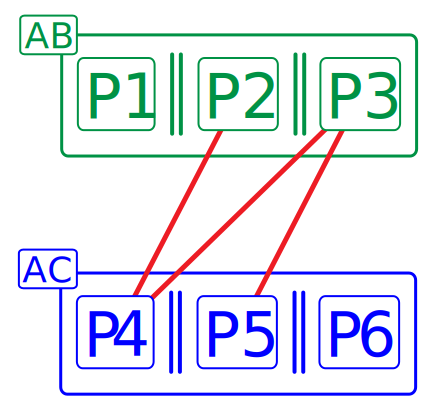
\includegraphics{img/parallel_patch_connected.png}
\caption{}
\end{figure}

Each connected component is either: 
\begin{enumerate}[1.]
\item
A connected component of size 1 from PPSet1 that does not conflict with anything in PPSet2 
\item
A connected component of size 1 from PPSet2 that does not conflict with
anything in PPSet1 
\item
A connected component of size greater than 1,
which we will refer to as a \emph{Maximal Conflict Set}, that contains
at least one patch from PPSet1 and at least one from PPSet2.
\end{enumerate}

Each Maximal Conflict Set (MCS) obeys the following properties: 
\begin{enumerate}[1.]
\item
$\forall$ patch, \emph{x}, in a given MCS, $\exists$ \emph{y} from the same
MCS where \emph{x} conflicts with \emph{y} such that \emph{x} and
\emph{y} are not from the same original set of parallel patches 
\item
$\forall$ patch, \emph{x}, in a given MCS, $\forall$ \emph{y} not in the MCS but in set
of connected components, \emph{x} does not conflict with \emph{y}
\end{enumerate}

\emph{(The term Maximal Conflict Set is used because if a single patch
is removed from a MCS then the second property no longer holds true.)}

After trying to merge the parallel patches, the result is a set of
non-conflicting \texttt{ParallelPatches} and any Maximal Conflict Sets
of \texttt{ParallelPatches}. Because non-conflicting patches all
reference the same original state (set of files), we can put all
non-conflicting patches immediately in parallel with one another. It
might not be obvious at first why we want to always get the Maximal
Conflict Set. Consider the following example:

\begin{figure}[Figure 5]
\centering
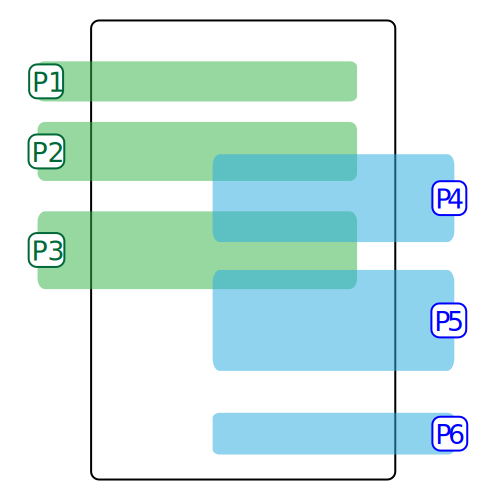
\includegraphics{img/parallel_patch_file.png}
\caption{}
\end{figure}

Patches P1, P2, and P3 together represent changing file A to file B and
patches P4, P5, and P6 represent changing file A to file C. We can see
from the diagram that P2 and P4 conflict, P4 and P3 conflict, and P3 and
P5 conflict because they have overlapping lines. However, when
displaying this as a conflict to the user, the entire set of conflicting
changes should be present so that the user can choose which lines ought
to be kept.

Once we have the Maximal Conflict Set, we can easily display this
conflict to the user. Because it is maximal, we know no other patch can
affect the interval of lines in the MCS. Therefore, we can simply
transform this conflict set into a single Patch (\texttt{ChangeHunk})
which replaces the total affected lines with the two possible
alternatives of applying the patches from the first set separated from
the result of applying the patches from the second on the given
interval.

Using our previous example, we compute the affected lines in the
original file A from P2 through P5. We then duplicate the affected
lines, applying P2 and P3 to one set and P4 and P5 to the other set. We
wrap the standardized markings
(``\textless{}\textless{}\textless{}\textless{}\textless{}'' ,
``====='',
``\textgreater{}\textgreater{}\textgreater{}\textgreater{}\textgreater{}'')
around the blocks to denote from where the changed lines originated.

\begin{figure}[Figure 6]
\centering
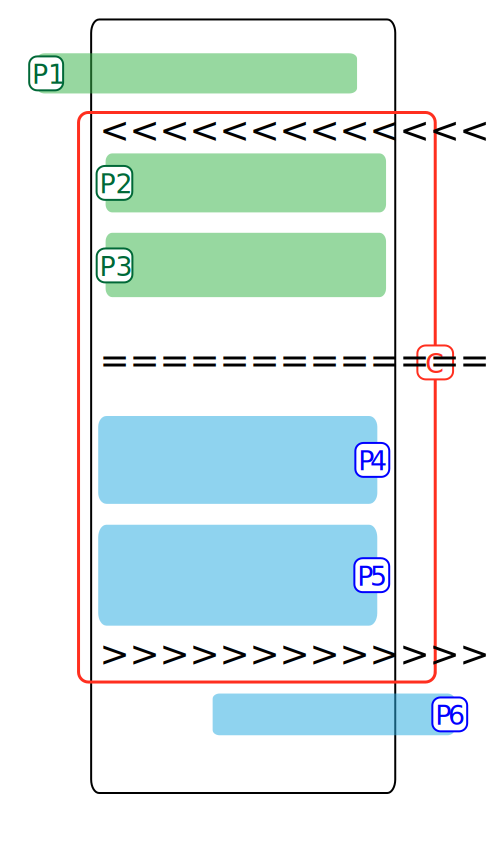
\includegraphics{img/parallel_patch_view_conf.png}
\caption{}
\end{figure}

We have now reduced the Maximal Conflict Set to a single ``Viewable
Conflict'' Patch. We can prove that this new patch will not conflict
with any other patches created so far.

\subsubsection{Proof that Viewable Conflict Patches are Non-Conflicting}

Assume a Maximal Conflict Set of patches, S, has been created from
merging parallel patch sets, PP\_1 and PP\_2, and that S can be reduced
to P\_vc. Let P* be another patch that conflicts with P\_vc not
contained in S but from PP\_1 or PP\_2. This means that P* modifies a
subset of the lines modified by P\_vc. Because all the lines modified by
P\_vc are modified by a patch that was originally found in S, P* must
conflict with a patch in S. If P* conflicts with a patch from S, then it
must also be in S by definition. Therefore, we have reached a
contradiction. =\textgreater{}\textless{}=.

Since we have proven that the reduction of a MCS into a single
ChangeHunk does not introduce new conflicts, we can place it in parallel
with the rest of the non-conflicting patches. We perform this Conflict
Reduction strategy by reducing all Maximal Conflict Sets until we only
have a set of parallel patches. This reduction is extremely powerful
because now we can simply sequence the parallel patches and apply it to
file for the user to resolve and no longer concern our model with
conflicts.

\section{Rebase}

Now that we can detect conflicts when merging two sets of parallel
patches and can reduce conflict sets into a viewable conflict patch, we
can easily design an algorithm for rebase which replays the commits of
one branch onto the other.

We assume a state based system in which each commit has a parent (except
for the root commit which is created when the repository is initialized)
and we can always find a common ancestor between any two commits. We
also require a function that can return the set of parallel patches
between two commits. ``Merging the commits'' then involves computing the
least common ancestor, finding the parallel patches between the lca and
each commit to be merged, and then merging the two sets of parallel
patches using the conflict detection algorithm described in the
preceding section.

The psuedocode for rebase appears below:

\begin{enumerate}[1.]
\item
  Compute the least common ancestor between the commit to rebase onto
  and the current head commit
\item
  Compute the list of commits (commitList) between the current head
  commit and the lca (including the head commit)
\item
  Change the head to the commit to rebase onto
\item
  While commitList has elements:

  \begin{enumerate}[a.]
  \item
    Merge the commit at the head of the list with the current head
    commit
  \item
    If there are no conflicts

    \begin{enumerate}[i.]
    \item
      Create a new commit with the head commit as its parent and make it
      the new head
    \item
      Recurse with the tail of commitList
    \end{enumerate}
  \item
    If there is a conflict

    \begin{enumerate}[i.]
    \item
      Reduce all the conflicts to a viewable patch
    \item
      Apply the patches to the files of the least common ancestor and
      notify the user of a conflict
    \item
      When the user resolves the conflict, create a commit from the
      patch between the lca and the current set of files
    \item
      Recurse with the tail of commitList
    \end{enumerate}
  \end{enumerate}
\end{enumerate}

Notice that in step 3.3.2 before we applied the conflicted patches we
had to restore the file system to the state of the least common ancestor
in order to properly apply the patches. The current state of the system
is referenced by the commit head, but all the parallel patches in our
simplified model reference the state of the least common ancestor.

\subsection{Rebase v. Merge}

Although at this point, our model assumes a similar state-based
representation such as found in git, we notably only detail an algorithm
for rebase. Both merge and rebase require comparing branches based on an
LCA, the commit at which the branches diverge. As mentioned, merge
requires multiple parents, while rebase requires the ability to walk,
commit-by-commit, from the end of a branch to the LCA. Meeting such two
requirements simultaneously results in difficulties, and the trouble
stems from multiple parents.

With multiple parents, there can be multiple LCAs and it is unclear what
is the definition of an LCA in this instance. First intuition might be
to define the LCA as the closest LCA, in number of commits away from
each. However, in the cases where there are multiple LCAs which are
\emph{all} equidistant in number of commits, there is no clear right
answer. In regards to merge, perhaps comparing against any LCA would
yield equivalent resulting merged commits since comparing against any
LCA would still allow the unique changes introduced in the individual
commits-to-be-merged to be detected.

As for rebase, things are exceedingly less clear. If rebase is viewed as
relocating the place at which a branch diverges, multiple LCAs mean
multiple points of divergence. Choosing any given LCA would yield a
difference sequence of replayed commits. Additionally, only in
relocating all the points at which a branch might diverge does the
number of branches decrease, a goal of combining different branches of
development.

Other VCS deal with this issue by removing commits with multiple parents
during a rebase. Such attempts are a work-around for ambiguity
surrounding the semantics actions of rebase and merge in the presence of
multiple parents. Git, for example, removes all commits with multiple
parents (resulting from a merge) when the user tries to rebase a branch
with that had a merge in it. Next, each of the many branches (since all
merge commits were removed), are merged in-turn onto the destination
branch. This is clearly not ideal, but it makes the best out of a
difficult situation. As for our model, we chose to only implement rebase
to avoid this difficulty and keep the model clean and concise.

\begin{figure}[Figure 7]
\centering
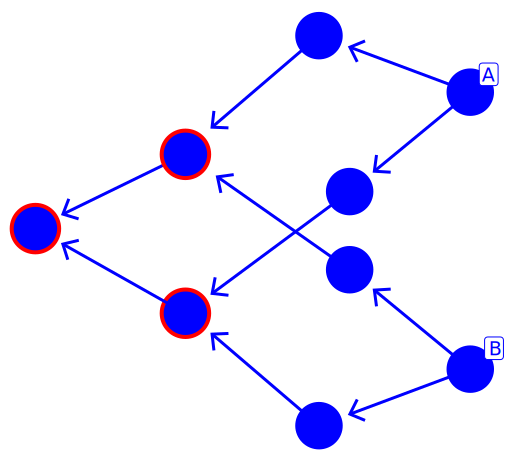
\includegraphics{img/mrg_rebase_3.png}
\caption{}
\end{figure}

\begin{figure}[Figure 8]
\centering
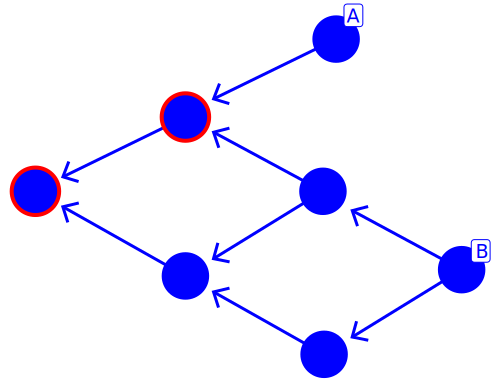
\includegraphics{img/mrg_rebase_2.png}
\caption{}
\end{figure}

\begin{figure}[Figure 9]
\centering
\mbox{
    \subfigure{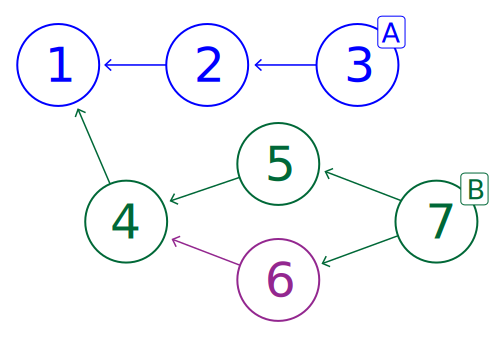
\includegraphics[width=3in]{img/git_crazy_graph.png}}
\quad
\subfigure{\includegraphics[width=3in]{img/git_crazy_rebase.png}}}
\caption{}
\end{figure}

\begin{figure}[Figure 10]
\centering
\caption{}
\end{figure}

\section{Testing}

One of the most well-known features of Haskell is the ability to
automatically test algebraic laws for pure functions using QuickCheck
(Claessen and Hughes 2000).

Most of our QuickCheck properties are devoted to conflict detection and
viewing conflicts as a single patch. We are able to verify the
properties of the non-conflicting patches and Maximal Conflict Sets
returned from our connected components algorithm for conflict detection.
Moreover, we can see the proof stating that viewable conflicts do not
create additional conflicts holds true.

One of the biggest challenges we faced when creating properties to test
our model of a VCS was creating meaningful test cases. This is commonly
found to be the most difficult aspect of using the testing framework
since incorrect instances of \texttt{Arbitrary} for the data types can
provide a false sense of security to the programmer. The parallel
patches merging algorithm relies on the fact that the two sets of
parallel patches all reference the same original state, and so in order
to properly test our algorithm, we had to preserve this assumption
throughout our tests.

We define two helper functions, \texttt{mkGoodPPatches} and
\texttt{mkGoodCHs} which allow us to generate non-conflicting parallel
patches and non-conflicting \texttt{ChangeHunks},respectively, when
given a file.

\begin{verbatim}
mkGoodCHs :: Int -> File -> Gen [ChangeHunk]
mkGoodPPatches :: File -> Gen ParallelPatches
\end{verbatim}

\texttt{mkGoodCHs} starts at a given offset in the file and arbitrarily
creates a new \texttt{ChangeHunk} for a random interval between the
current offset and the end of the file, and recursively creates more
\texttt{ChangeHunks} until hitting the end of the file.
\texttt{mkGoodPPatches} takes a file and either calls
\texttt{mkGoodPPatches} or returns a singleton list containing a
\texttt{RemoveFile} for the file (this case has a lesser probability.
Notice that \texttt{mkGoodPPatches} never returns any
\texttt{CreateFile}, this is because we cannot ever have two patches in
parallel where one is a \texttt{CreateFile} and the other is not a
\texttt{CreateFile}.

All of this is combined together in an instance of arbitrary for a new
type, \texttt{PPatchesFromFiles}, which is simply a wrapper around two
collections of patches in parallel. We can simply generate patches by
mapping over arbitrary files and occasionally generating
\texttt{CreateFile} patches along the way.

With this instance, we can now test the properties of our conflict
detection algorithm successfully.

\section{Future work}

While the representation of patches allows for simplified conflict
detection and an understandable and predictable algorithm for rebase, we
hope to continue to expand and improve upon our work. In greater detail,
we hope to formalize the differences between parallel and sequential
patches by showing under which operations these data types are monoidic.
This could provide greater insight into why conflict detection and
merging of patches appears to have a great disparity in the complexity
of the algorithm and illuminate further testable algebraic laws for our
code.

We would also like to explore a slightly more sophisticated rebase
algorithm which appears to be employed by state of the art version
control systems such as git. Consider the following example: if commit E
relies on changes made in commit D, and upon replaying D upon C a
conflict occurs, git knows to update the chosen resolution in E's
reliance on D. This is a nice usability feature of git which reduces the
number of conflicts a user has to solve. More research is needed into
understanding the precise semantics of this feature.

Lastly, we would like to explore further the possibility of
incorporating a merge operation into our simplified version control
system. Ultimately, this involves tackling the problem of multiple
parents and the potential for an unclear least common ancestor.

\section{Conclusions}

We have identified a need in the academic literature for a simple model
of a version control system to better understand the difficult and
interesting challenges that implementors face when building a version
control system. In addition, we recognize that implementors want to
ensure that complicated operations such as conflict detection, merge,
and rebase are well behaved for their users under a variety of
conditions. Being able to reason about such complex operations is the
first step in achieving such a goal.

Our work establishes a model of a version control system in which
changes between states in a repository are represented as patches in
parallel. Detecting conflicts between two sets of parallel patches from
a common ancestor and merging them into a single set of parallel patches
can be achieved with a simple and graphing algorithm. This presents a
significant improvement over previous work, where little has been done
for state-based systems. Building off of our ability to merge parallel
patches, implementing rebase becomes fairly straightforward. With rebase
in hand, we are now able to view the challenges associated with
developing a system that incorporates both of these operations, leaving
open questions to how specific examples of multiple least common
ancestors should be handled.

We believe this model to particularly useful in designing a version
control system that is easier to understand and reason about. To support
these claims, we have implemented a state-based version control system
using this representation and the algorithms for conflict detection and
rebase. We call the system \emph{nor}. We hope to continue to expand
upon our model and implementation over time to better understand some of
the very interesting challenges associated with version control.

\section{Source}

The source code for nor can be found at
\href{https://github.com/jmont/nor}{github.com/jmont/nor}. This writing
deals with the code tagged `v0.1'.

\section{References}

Claessen, Koen; Hughes, John. \emph{QuickCheck: a Lightweight Tool for
Random Testing of Haskell Programs}. 2000. Dagit, Jason. ``Darcs Patch
Theory''. \emph{The Monad Reader}. November 2007. Roundy, David.
``Theory of Patches''. Appendix A in Darcs 2.1 user manual. April 2009.
Wiegley, John. ``Git from the Bottum Up''.
\url{http://ftp.newartisans.com/pub/git.from.bottom.up.pdf}. December
2009.

\end{document}
